Prvi problem koji sam definirao je problem rekonstrukcije slike s dodanim šumom.
Promatramo sliku, definiranu kao matrica $I$ veličine $w \times h$ gdje za svaki element $x$ na koordinatama $(i, j)$ vrijedi $x_{(i, j)} \in [0, 255]$ što predstavlja intentzitet boje od crne prema bijeloj. \\
Sintetički šum koji sam dodao vrste \emph{"Salt and pepper"} odnosno soli i papra nazvan je tako jer određeni postotak nasumičnih vrijednosti postavi na bijelu ili crnu boju (slika \ref{fig:salt_pepper_example}).

\begin{figure}
	\centering
	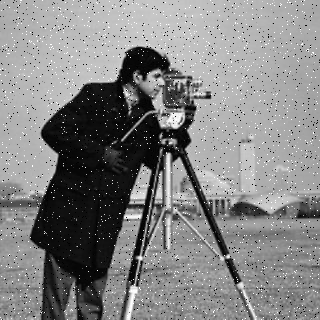
\includegraphics[width=0.5\linewidth]{Experiments/GrainRemoval/input_example.png}
	\caption{Primjerak fotografije s $5\%$ šuma soli i papra}
	\label{fig:salt_pepper_example}
\end{figure}

Postotak slike na koji sam odlučio primjeniti šum je $5\%$, slično kao i \cite{cgp_image_processing} i \cite{Sekanina2011}.
U nastavku rada također ću predstaviti rezultate na većem postotku šuma od $40\%$.

Cilj eksperimenta je evoluirati filter $f(x): [0, 255]^8 \rightarrow [0, 255]$ koristeći konvolucijske metode i CGP koji će od oštećene slike $D$ reproducirati novu $Y = f(D)$ što bližu neoštećenom originalu $I$.
$$
\min_{Y, i, j} |Y_{(i, j)} - I_{(i, j)}|
$$
Iz susjedstva svake vrijednosti želimo dobiti što precizniju promatranu vrijednost. \\
Polazišna pretpostavka je ta da su susjedne vrijednosti na slici u međusobnoj korelaciji do određene mjere te mogu pomoći u zaključivanju originalne vrijednosti.
Problem koji se može javiti je da u promatranom susjedstvu također imamo vrijednost koja je šum, što narušava pretpostavku korelacije.
Navedeni problem je zanemaren te je CGP-u ostavljeno kao problem koji treba riješiti bez ljudskog znanja.

Jezgra $\omega$ koju sam odlučio koristiti je veličine $3 \times 3$, koja promatra $Moore$-ovo susjedstvo (\cite{jakobovic}).
\[
	\omega_{(i, j)}
	=
	\begin{bmatrix}
		x_{(i - 1, j - 1)} && x_{(i - 1, j)} && x_{(i - 1, j + 1)}\\
		x_{(i, j - 1)} && && x_{(i, j + 1)}\\
		x_{(i + 1, j - 1)} && x_{(i + 1, j)} && x_{(i + 1, j + 1)}
	\end{bmatrix}
\]
Razmišljanje iza korištenja jezgre koja ne koristi središnju, promatranu vrijednost je što tu vrijednost upravo pokušavamo predvidjeti, a njena vrijednost, posebice ako je šum ne smije imati utjecaja.
Detaljniji prikaz djelovanja i rezultata mooreove jezgre vidljiv je na ilustraciji \ref{fig:moore_example}

\begin{figure}
	\centering
	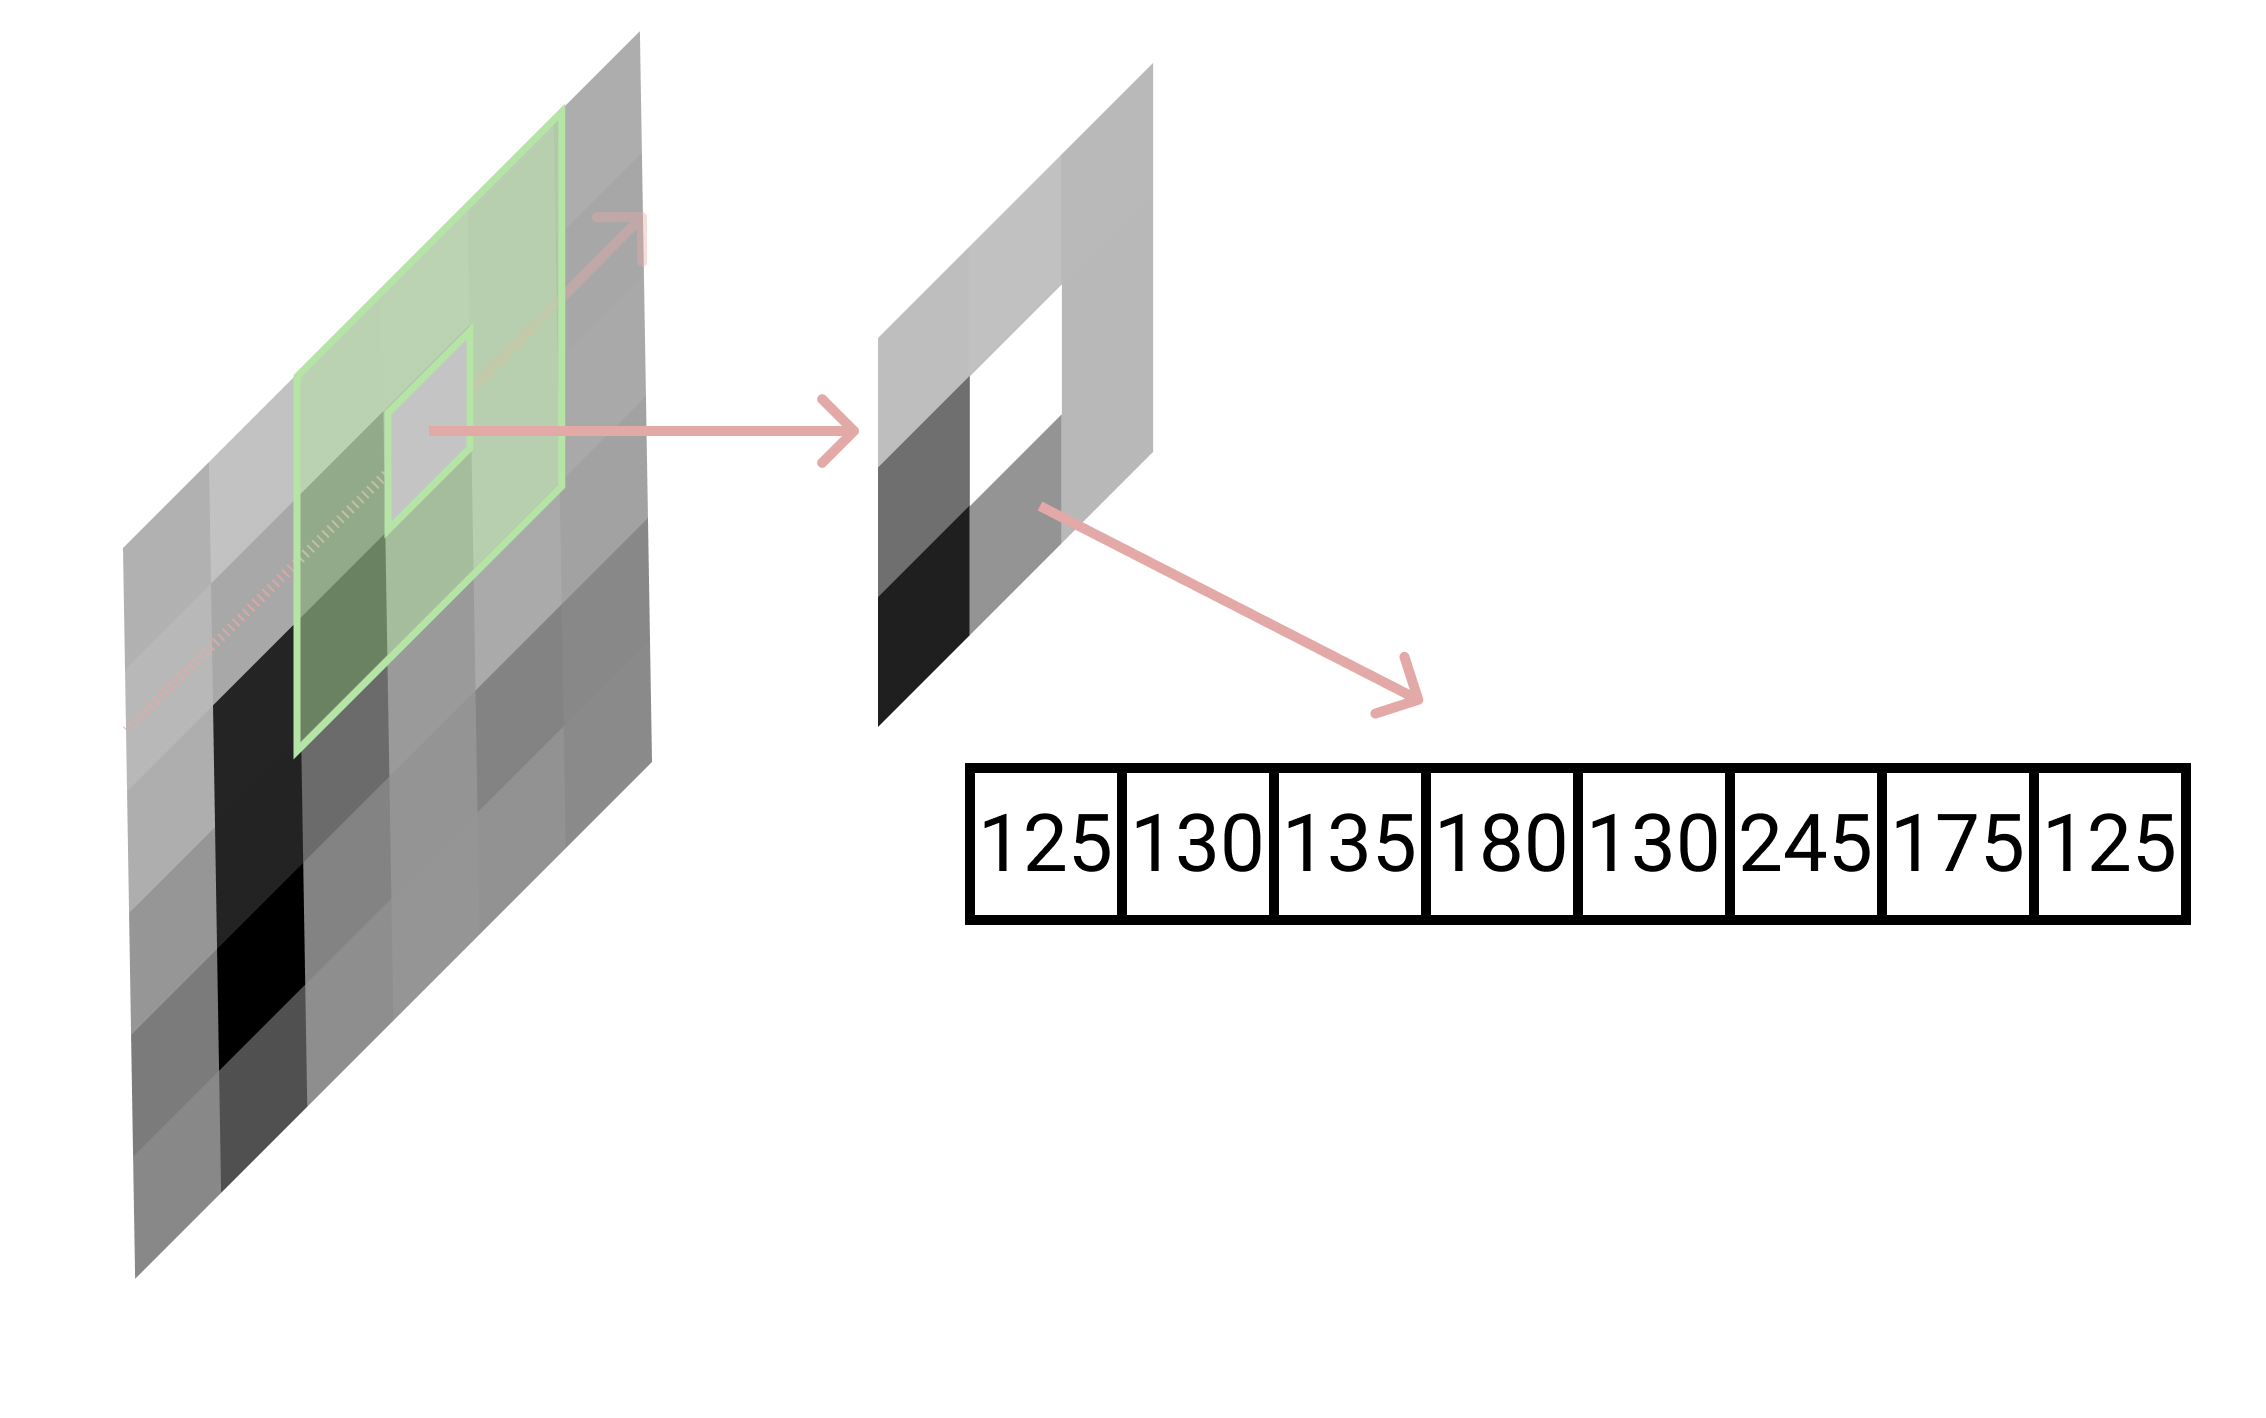
\includegraphics[width=0.8\linewidth]{Illustrations/moore.png}
	\caption{Primjer čitanja slike mooreovom jezgrom te transformacija iz preuzetog dijela slike u vektor vrijednosti koristivih CGP-u}
	\label{fig:moore_example}
\end{figure}

Za rješavanje problema potrebno je definirati prikladne uvjete zaustavljanja.
Kondicijska funkcija koju sam odabrao temeljena je na $L1$ pogrešci, odnosno,
\begin{gather*}
err = \sum_{i=1}^{n} |y_{cgp} - y_{skup\ podataka}| \\
kondicija = \frac{1}{err}
\end{gather*}
gdje je $y_{cgp}$ vrijednost koju računa CGP a $y_{skup\ podataka}$ vrijednost koju želimo predvidjeti i biti joj što bliže.
Jezgrom konvolucije prolaziti će se cijelom slikom čitajući vrijednosti osam susjeda pravilom opisanim gore, pretvarajući na kraju očitanu matricu u vektor.
Vektor se predaje CGP jedinki koja na temelju ulaza i operacija koje se izvode u skrivenim slojevima računa izlaz.
Konačno, ideja je minimizirati $L1$ pogrešku $err$, odnosno, dobiti jedinku s najvećom kondicijom.

\subsubsection{Postavke}
Početne slike u punoj su veličini $256 \times 256$.
Na slike je programski dodan nasumičan šum na $5\%$ vrijednosti.
Zbog polinomijalnog rasta broja vrijednosti s rastom slike, promatrani su podskupovi veličine $30 \times 30$.
Time nastaje skup podataka od $900$ vrijednosti.
Slike \ref{fig:lena_subsets} prikazuju cijelu sliku, podskup i jednu vrijednost konvolucijske jezgre iz podskupa.

\begin{figure}
	\centering
	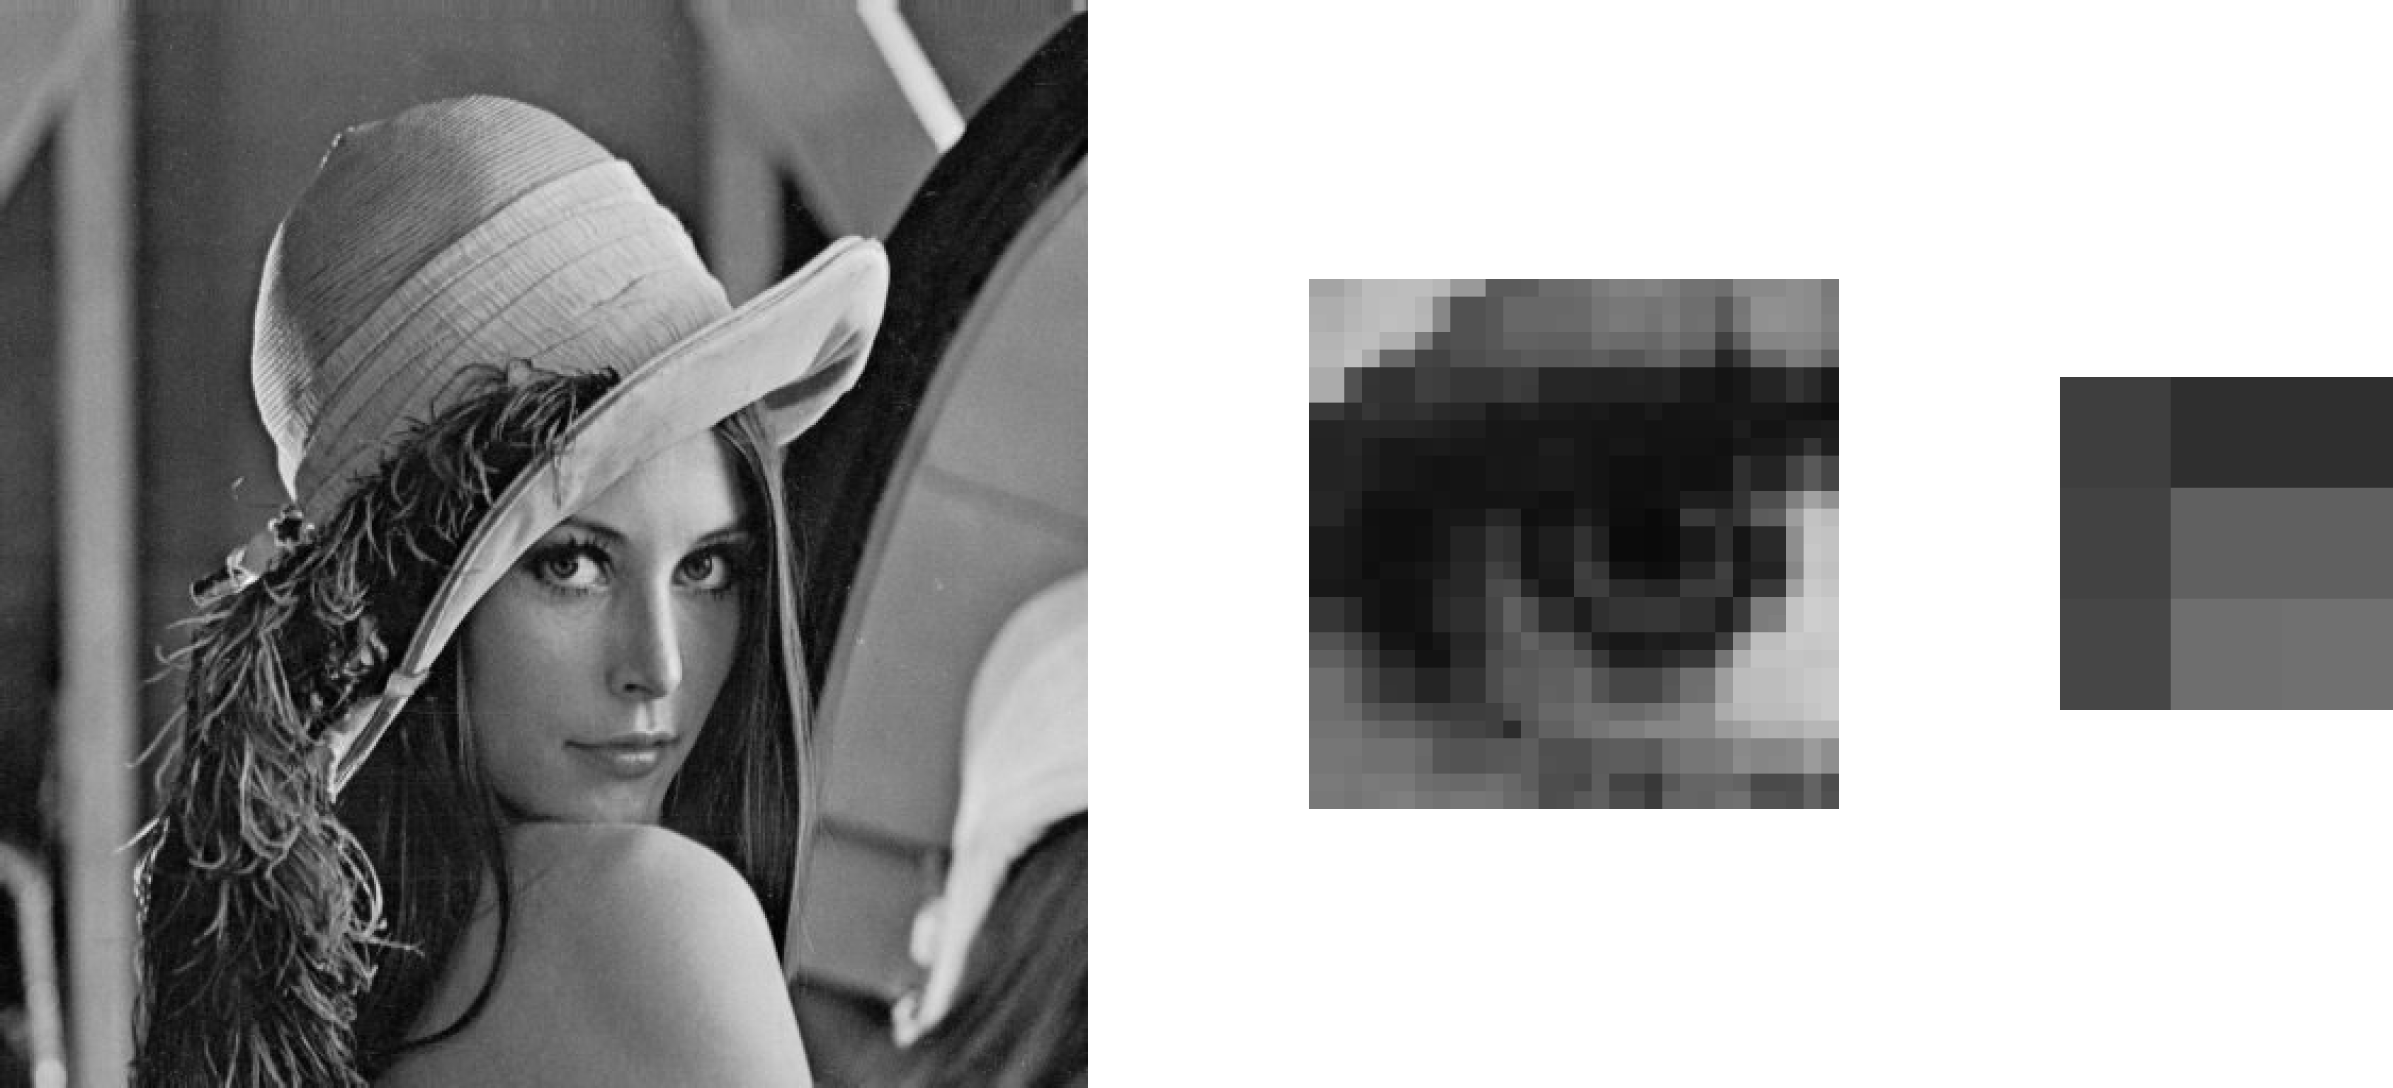
\includegraphics[width=0.8\textwidth]{Experiments/GrainRemoval/lena_subsets.png}
	\caption{Prikaz cijele fotografije Lene, jedan promatrani podskup veličine $30 \times 30$ i jedna vrijednost jezgre veličine $3 \times 3$ iz podskupa.}
	\label{fig:lena_subsets}
\end{figure}

Fotografije \ref{fig:sp_samples} prikazuju slike koje su se koristile u pojedinim fazama.

Arhitektura CGP-a definirana je s $20$ funkcijskih čvorova raspodjeljenih kao $2 \times 10$, odnosno, $2$ retka i $10$ stupaca.
Kako bi se sačuvala kompleksnost modela, najveći broj stupaca unazad koje pojedini čvor može čitati ($L$), definiran je kao $L = 3$.
Također, izlazni čvorovi (u ovom slučaju $1$) mogu čitati vrijednosti samo iz posljednjeg stupca.

Svaki eksperiment bio je ponovljen 30 puta.
Odabrani algoritam je $1 + \lambda$, $\lambda = 4$.
Koristi se samo operator mutacije koji mutira 1 aktivni gen po iteraciji.
Dozvoljeno je najviše $500$ generacija, odnosno, $2000$ evaluacija.
Također, u slučaju pada greške ispod $0.005$ postupak se zaustavlja.
Tablica \ref{table:sp_function_set} prikazuje funkcije koje su se mogle koristiti u čvorovima.
Funkcije su odabrane na način da izlaz uvijek odgovara skupu $[0, 255$] iako je dozvoljeno manje, odnosno, veće vrijednosti vratiti na najbližu dozvoljenu rubnu vrijednost koristeći jednakost $f(x) = max(min(f(x), 255), 0)$.

\begin{table}
	\centering
	\begin{tabular}{||c c c c||}
		\hline
		Adresa funkcije & Funkcija & Broj ulaza & Broj izlaza \\ [0.5ex]
		\hline \hline
		0 & $max$ & 8 & 1\\
		1 & $min$ & 8 & 1\\ 
		2 & $avg$ & 8 & 1\\ 
		3 & $mean$ & 8 & 1\\ 
		4 & $sum\ mod\ 256$ & 8 & 1\\ 
		5 & $\sqrt{sum}$ & 8 & 1\\ 
		6 & $max - min$ & 8 & 1\\ [1ex]
		\hline
	\end{tabular}
	\caption{Funkcije korištene u postupku micanja šuma sa slike}
	\label{table:sp_function_set}
\end{table}

\begin{figure}
	\caption{Fotografije na koje će biti primjenjen šum korištene u fazi učenja, validacijskoj i testnoj fazi}
	\begin{subfigure}[t]{0.45\textwidth}
		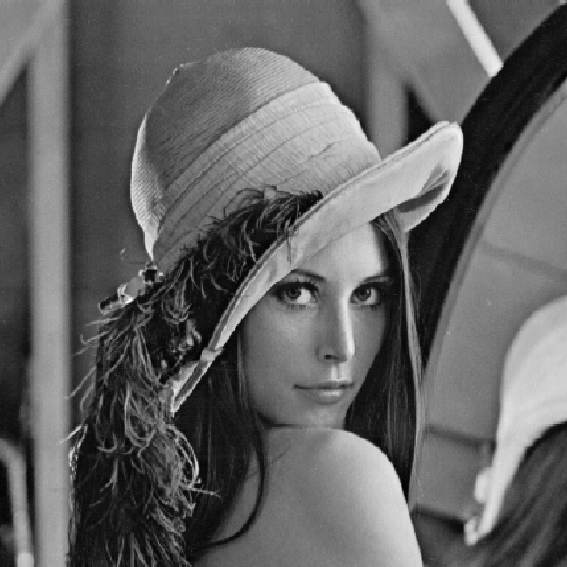
\includegraphics[width=\textwidth]{Experiments/GrainRemoval/lena.png}
		\caption{Lena, fotografija na kojoj će se izvoditi učenje i na temelju koje će se model korigirati}
		\label{fig:sp_train_sample}
	\end{subfigure}
	\begin{subfigure}[t]{0.45\textwidth}
		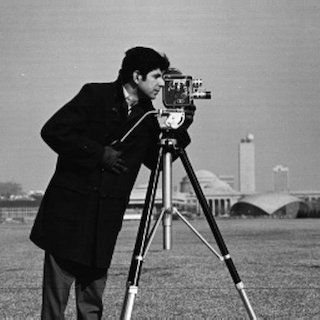
\includegraphics[width=\textwidth]{Experiments/GrainRemoval/cameraman.jpg}
		\caption{Kamerman, fotografija na temelju koje će se računati validacijska kondicija CGP-a. Na temelju ove fotografije model se ne korigira}
		\label{fig:sp_val_sample}
	\end{subfigure}
	\begin{subfigure}[t]{0.45\textwidth}
		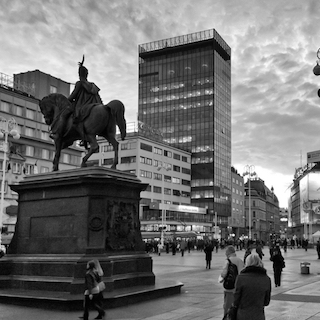
\includegraphics[width=\textwidth]{Experiments/GrainRemoval/trg.jpg}
		\caption{Trg bana Jelačića, fotografija koja će se predati konačnom modelu u testnoj fazi imitirajući tako problem iz \emph{stvarnog svijeta}}
		\label{fig:sp_test_sample}
	\end{subfigure}
	\label{fig:sp_samples}
\end{figure}

\subsubsection{Rezultati}
Rezultati micanja šuma prikazani su na slikama \ref{fig:sp_result_grid}.
Posebno je zanimljivo vidjeti posljednji redak gdje je prikazana razlika između željene i dobivene fotografije.
Vidljivo je i očekivano da je najveći problem nastao na područjima fotografije gdje su velike razlike u susjedstvu, točnije, rubovima.
Na fotografiji kamermana može se jasno pratiti kontura tijela i fotoaparata.
Najveća razlika očekivano je najvidljivija na testnoj slici koja je istovremeno i najdetaljnija.

\begin{figure}
	\centering
	\caption{Fotografije iz faze za učenje, validacijske i testne faze prije i nakon micanja šuma CGP-om. Na dnu je također prikazana razlika dobivene slike i one željene.}
	\begin{subfigure}[t]{0.32\textwidth}
		\includegraphics[width=\textwidth]{Experiments/GrainRemoval/noisy_lena.png}
		\caption{Lena s $5\%$ šuma}
	\end{subfigure}
	\begin{subfigure}[t]{0.32\textwidth}
		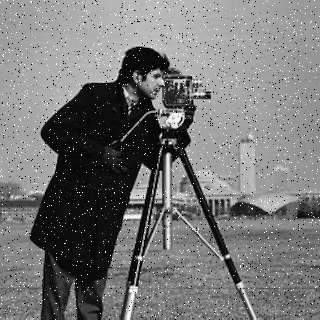
\includegraphics[width=\textwidth]{Experiments/GrainRemoval/cameraman_noisy.png}
		\caption{Kamerman s $5\%$ šuma}
		\label{fig:sp_samples_camerman}
	\end{subfigure}
	\begin{subfigure}[t]{0.32\textwidth}
		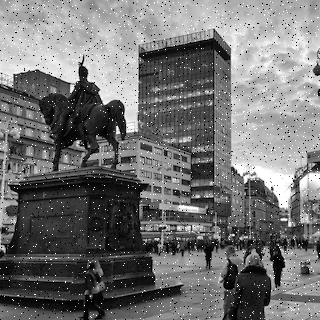
\includegraphics[width=\textwidth]{Experiments/GrainRemoval/trg_noisy.png}
		\caption{Testna slika s $5\%$ šuma}
	\end{subfigure}
	\begin{subfigure}[t]{0.32\textwidth}
		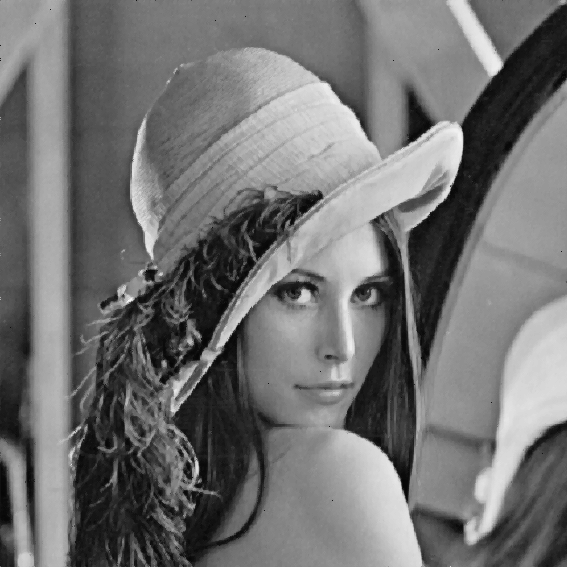
\includegraphics[width=\textwidth]{Experiments/GrainRemoval/sp_output.png}
		\caption{Lena nakon prolaska kroz dobiveni filter}
	\end{subfigure}
	\begin{subfigure}[t]{0.32\textwidth}
		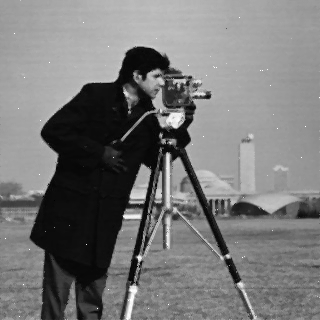
\includegraphics[width=\textwidth]{Experiments/GrainRemoval/cameraman_out.png}
		\caption{Kamerman nakon prolaska kroz dobiveni filter}
	\end{subfigure}
	\begin{subfigure}[t]{0.32\textwidth}
		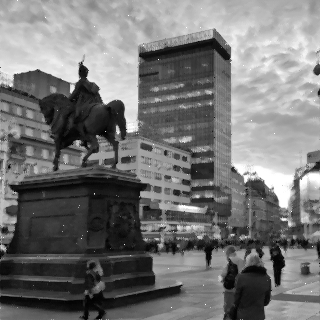
\includegraphics[width=\textwidth]{Experiments/GrainRemoval/trg_out.png}
		\caption{Testna slika s maknutim šumom}
	\end{subfigure}
	\begin{subfigure}[t]{0.32\textwidth}
		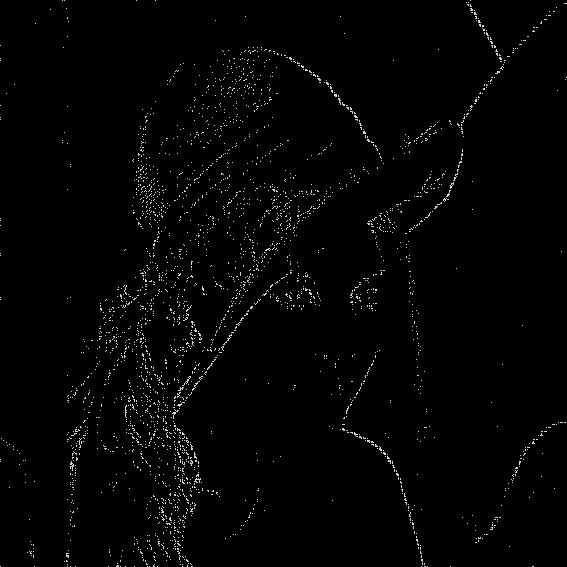
\includegraphics[width=\textwidth]{Experiments/GrainRemoval/sp_diff_train.png}
		\caption{Razlika između dobivene i željene fotografije za učenje}
	\end{subfigure}
	\begin{subfigure}[t]{0.32\textwidth}
		
\includegraphics[width=\textwidth]{Experiments/GrainRemoval/sp_diff_val.png}
		\caption{Razlika između dobivene i željene validacijske fotografije}
	\end{subfigure}
	\begin{subfigure}[t]{0.32\textwidth}
		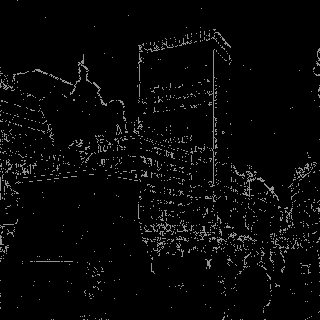
\includegraphics[width=\textwidth]{Experiments/GrainRemoval/sp_diff_test.png}
		\caption{Razlika između dobivene i željene testne fotografije}
	\end{subfigure}
	\label{fig:sp_result_grid}
\end{figure}

Osim grafičkog prikaza rezultata i subjektivne procjene kvalitete rezultata grafovi \ref{fig:sp_train_val_graph_1} i \ref{fig:sp_train_val_graph_2} prikazuju kretanje greške na skupu za učenje i validacijske greške tijekom iteracija algoritma za dva nasumična pokretanja.
Odabrana jedinka je ona s grafa \ref{fig:sp_train_val_graph_1} jer uz to što ima validacijsku pogrešku usporedivu s jedinkom s grafa \ref{fig:sp_train_val_graph_2} nije pokazala znakove prenaučenosti.
Također, prikazana $L1$ pogreška je prilikom izračuna dodatno podjeljena s $255$, odnosno $err = \frac{err_{L1}}{255}$, kako bi se vrijednosti dobile unutar skupa $[0, 1]$.

\begin{figure}
	\centering
	\caption{Grafovi kretanja $L1$ pogreške kroz iteracije algoritma}
	\begin{subfigure}[t]{0.48\textwidth}
		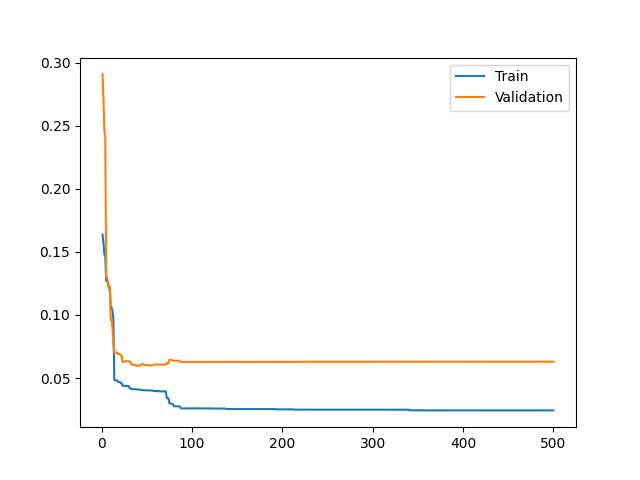
\includegraphics[width=\textwidth]{Experiments/GrainRemoval/sp_train_val_1.png}
		\caption{Primjer kretanja $L1$ pogreške}
		\label{fig:sp_train_val_graph_1}
	\end{subfigure}
	\begin{subfigure}[t]{0.48\textwidth}
		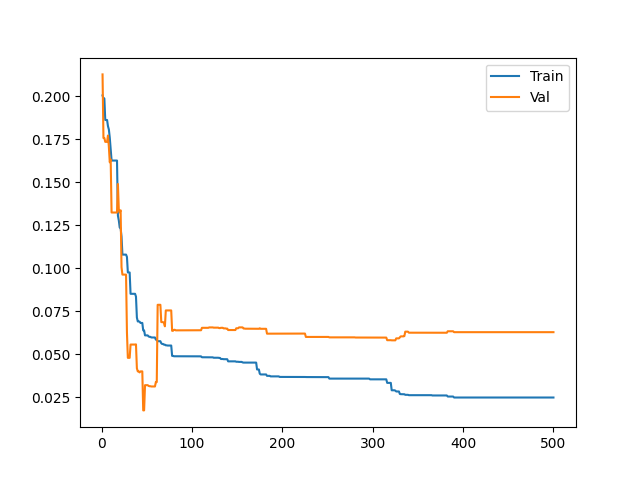
\includegraphics[width=\textwidth]{Experiments/GrainRemoval/sp_train_val_2.png}
		\caption{Primjer kretanja $L1$ pogreške s vidljivim nastankom prenaučenosti nakon $70.$ iteracije}
		\label{fig:sp_train_val_graph_2}
	\end{subfigure}
	\label{fig:sp_train_val_graph}
\end{figure}

Zanimljivo je pogledati korisnost pojedinih funkcija vidljivu u tablici \ref{table:sp_function_quality}.
Prvi stupac prikazuje funkciju privremeno izbačenu iz skupa, dok drugi stupac prikazuje utjecaj nedostatka te funkcije na rezultat.
Svako mjerenje izvršeno je 10 puta te je uzet medijan kao vrijednost koja se koristi u izračunu.
Vidljivo je da izbacivanje funkcija $min$ ili $max$ poboljšava ponašanje eksperimenta, ukazujući na to da nisu bitne ili štete, dok funkcija $mean$ uvelike doprinosi algoritmu.

\begin{table}
	\centering
	\begin{tabular}{||c c||}
		\hline
		Izbačena funkcija & Utjecaj na pogrešku (manje je bolje)\\ [0.5ex]
		\hline \hline
		$max$ & $0.9103$\\ 
		$min$ & $0.9315$\\ 
		$max - min$ & $0.9356$\\ 
		$sum mod 256$ & $0.9857$\\ 
		$\bm{osnova}$ & $\bm{1.0}$\\ 
		$avg$ & $1.0934$\\ 
		$\sqrt{sum}$ & $1.2075$\\ 
		$mean$ & $1.3499$\\ [1ex]
		\hline
	\end{tabular}
	\caption{Analiza doprinosa pojedinih funkcija pri micanju šuma. Osnovno mjerenje dozvoljava sve funkcije iz skupa.}
	\label{table:sp_function_quality}
\end{table}

\subsubsection{Rad s većim postocima}
Definirani CGP nije pokazao dobre rezultate u micanju šuma sa slike $40\%$ prekrivene šumom.
CGP koji se pokazao korisnim koristio je arhitekturu $2 \times 20$ s parametrom $L = 2$.
Skup funkcija bio je isti kao u radu s manjim postocima (tablica \ref{table:sp_function_set}).

Također, koristile su se fotografije za učenje, validaciju i testiranje.
Razlika s prošlim eksperimentom je što je u ovom slučaju za fotografiju za učenje i validaciju korištena ista fotografija s dva odvojena podskupa (Slika \ref{fig:large_sp_train_val_illustration}, a kao testna slika fotografija kamermana (Fotografija \ref{fig:sp_samples_camerman}

\begin{figure}
	\centering
	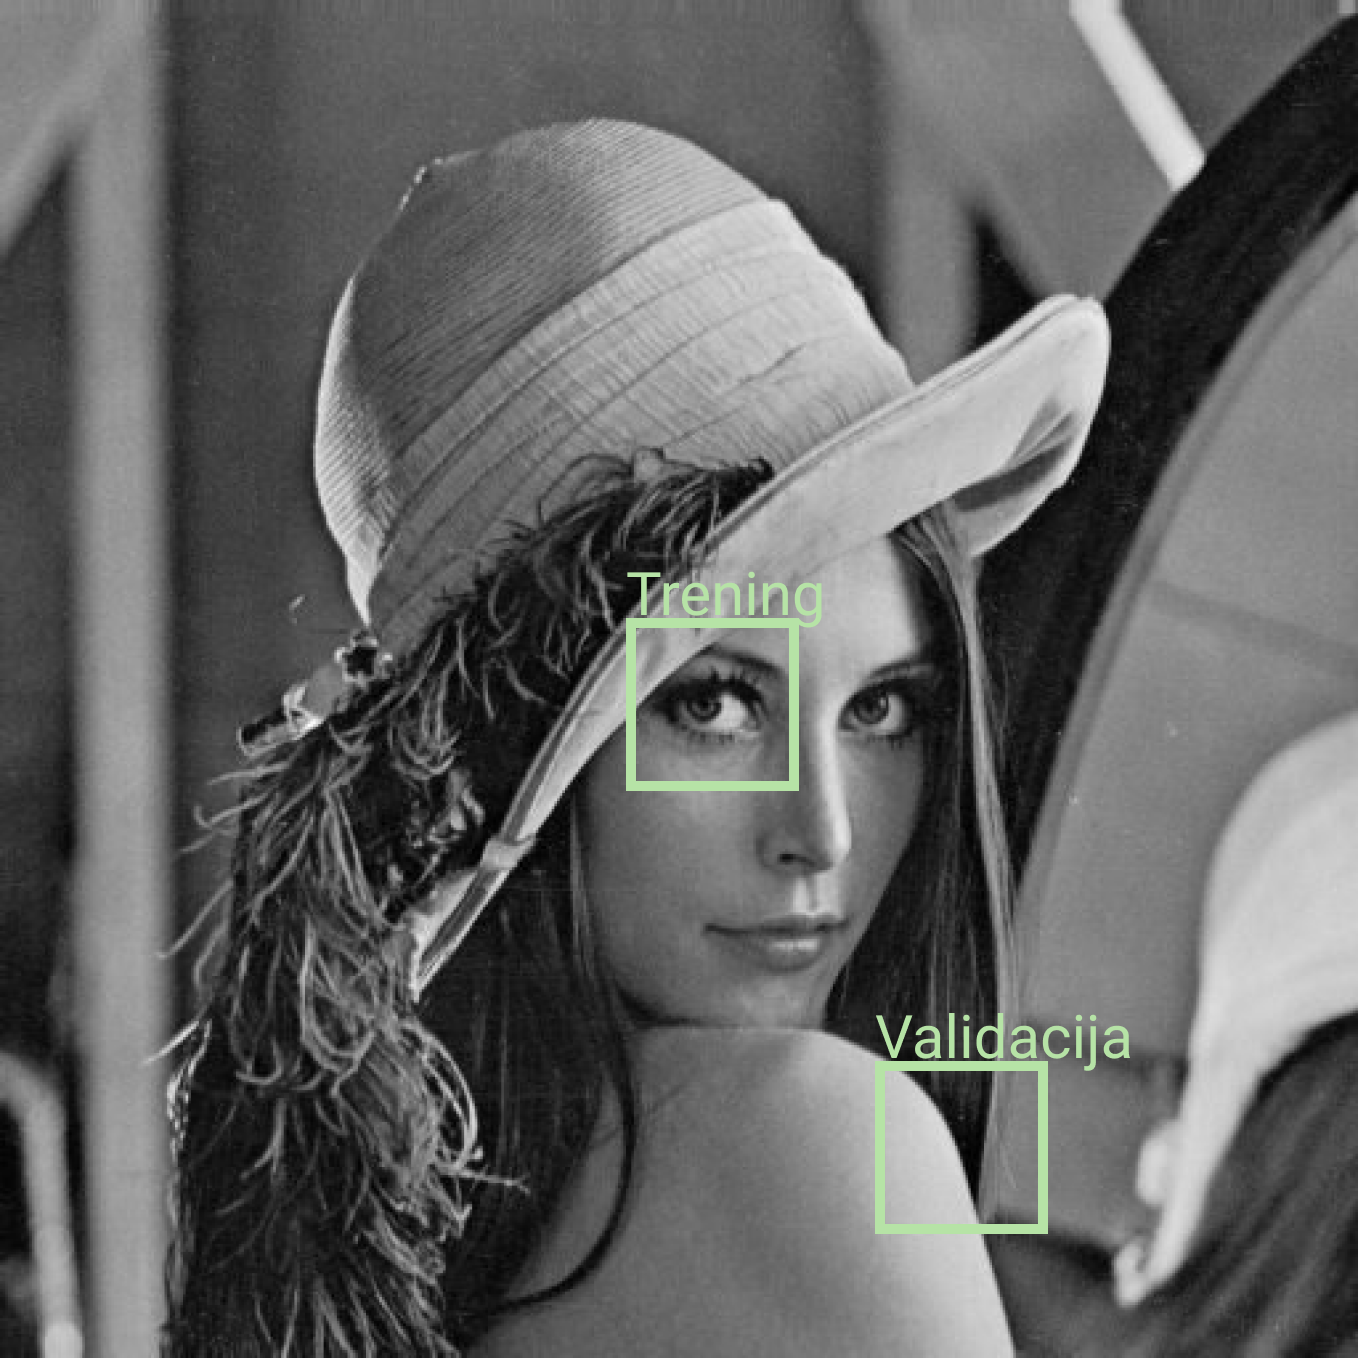
\includegraphics[width=0.7\linewidth]{Experiments/LargeGrainRemoval/large_sp_train_val.png}
	\caption{Trening i validacijski podskup fotografije Lene}
	\label{fig:large_sp_train_val_illustration}
\end{figure}

Rezultati su prikazani na slikama \ref{fig:large_sp_result_grid}, dok je kretanje $L1$ pogreške vidljivo na grafu \ref{graph:large_sp_train_val_loss}.
Očekivano testna slika pokazuje nešto lošije performanse u usporedbi sa slikom za učenje, odnosno, validacijskom slikom, no pokazuje poboljšanja u odnosu na početnu sliku.
Također, zanimljivo je što višestruko pokretanje micanja šuma na istoj fotografiji ne proizvodi bolje ili nešto drukčije fotografije nakon prvog prolaska kroz cijelu sliku.

\begin{figure}
	\centering
	\caption{Fotografije lene i fotografa prije i poslije micanja šuma koji prekriva $40\%$ slike}
	\begin{subfigure}[t]{0.35\textwidth}
		\includegraphics[width=\textwidth]{Experiments/LargeGrainRemoval/noisy_lena.png}
		\caption{Lena s $40\%$ šuma}
	\end{subfigure}
	\begin{subfigure}[t]{0.35\textwidth}
		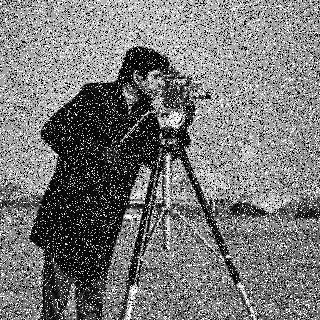
\includegraphics[width=\textwidth]{Experiments/LargeGrainRemoval/noisy_camerman.png}
		\caption{Kamerman s $40\%$ šuma}
	\end{subfigure}
	\begin{subfigure}[t]{0.35\textwidth}
		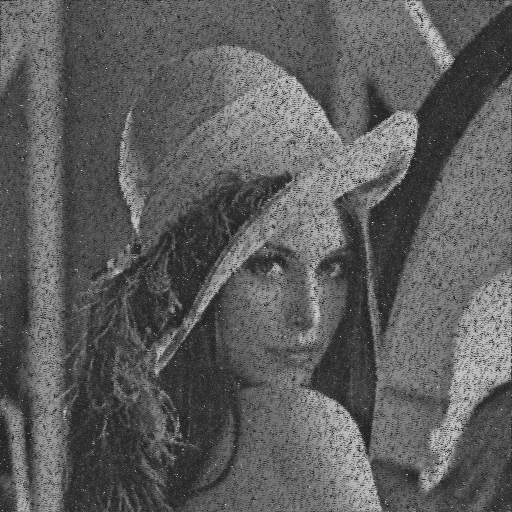
\includegraphics[width=\textwidth]{experiments/largegrainremoval/lena_fixed.png}
		\caption{lena s uklonjenim šumom}
	\end{subfigure}
	\begin{subfigure}[t]{0.35\textwidth}
		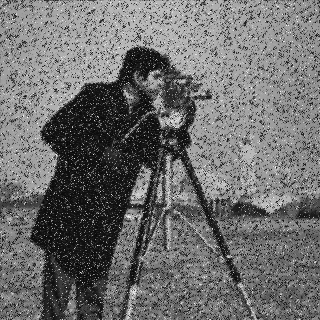
\includegraphics[width=\textwidth]{experiments/largegrainremoval/camerman_fixed.png}
		\caption{kamerman s uklonjenim šumom}
	\end{subfigure}
	\label{fig:large_sp_result_grid}
\end{figure}

\begin{figure}
	\centering
	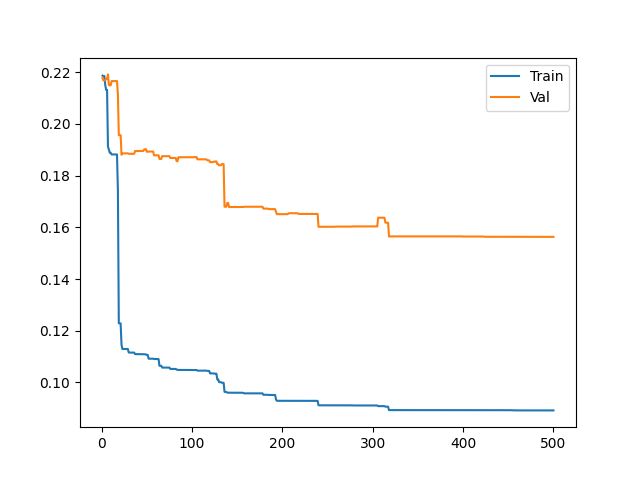
\includegraphics[width=0.6\linewidth]{Experiments/LargeGrainRemoval/lgr_errs.png}
	\caption{Kretanje $L1$ pogreške na skupovima za učenje i validaciju kroz iteracije algoritma}
	\label{graph:large_sp_train_val_loss}
\end{figure}
